\newpage
\chapter{Cambio de Variables}
Dada una ecuación diferencial de primer orden en forman normal
\begin{equation*}
    \dfrac{dx}{dt} = x' = f(t,x)
\end{equation*}

mediante una función 
\Func{f}{D}{\mathbb{R}}{(t,x)}{f (t,x)}
continua definida en $D\subseteq \mathbb{R}^2$ un conjunto abierto y conexo, nuestro objetivo será, dado un cambio de variable por dos ecuaciones
\begin{equation*}
    \left\{\begin{array}{rl}
        s=\varphi_1(t,x) \\
        y = \varphi_2(t,x)
    \end{array}\right.
\end{equation*}

con 
\Func{\varphi_1,\varphi_2}{D}{\mathbb{R}}{(t,x)}{\varphi_1(t,x), \varphi_2(t,x)}
cambiar tanto la expresión de la ecuación diferencial como el dominio para facilitar la resolución del mismo, mediante una aplicación
\Func{\varphi= (\varphi_1,\varphi_2)}{D}{D_1}{(t,x)}{(s,y)}
con $D_1\subseteq \mathbb{R}^2$ abierto y conexo, que nos lleve a una ecuación diferencial
\begin{equation*}
    \dfrac{dy}{ds} = \hat{f} (s,y)
\end{equation*}

para cierta función
\Func{\hat{f}}{D_1}{\mathbb{R}}{(s,y)}{\hat{f} (s,y)}
Y será de nuestro interés buscar la expresión de dicha $\hat{f}$.\\

Nos preguntamos también por las condiciones que tenemos que exigirle a dicha $\varphi$ para que el cambio de variable sea bueno:
\begin{enumerate}
    \item Que $\varphi$ sea biyectiva, o equivalentemente, que tenga inversa $\psi = \varphi^{-1}$, para poder deshacer el cambio de variable.
    \item Que podamos hacer cálculo diferecial en ambos lados y que podamos transportarlo, es decir, que tanto $\varphi$ como $\psi$ sean de clase $C^1$.
    \item Además, también tendremos que buscar cómo poner $y$ en función de $s$, y exigir hipótesis para que podamos hacerlo.
\end{enumerate}

\begin{definicion}[Difeomorfismo]
    Sea $r\in \mathbb{N}$, una aplicación $f:A\rightarrow B$ es un \newline$C^r$-difeomorfismo si $f$ es de clase $C^r(A)$, biyectiva y su inversa $f^{-1}$ es de clase $C^r(B)$.
\end{definicion}
De esta forma, nos interesará que $\varphi$ sea un $C^1$-difeomorfismo, para que se cumplan los dos primeros puntos de la enumeración anterior\footnote{Recordamos que una función de $\mathbb{R}^2$ sea de clase $C^1$ significa que podemos hacer sus derivadas parciales respecto a las dos variables y que ambas son continuas.}.\\

A continuación, realizaremos un razonamiento informal con la finalidad de comprobar qué pasará al realizar el cambio de variable, para luego formalizar el mismo.\\

Volviendo a la situación inicial, nos encontrábamos ante una ecuación de la forma
\begin{equation*}
    \dfrac{dx}{dt} = f(t,x)
\end{equation*}
y nos disponíamos a realizar un cambio de variable
\begin{equation*}
    \left\{\begin{array}{rl}
        s = \varphi_1(t,x) \\
        y = \varphi_2(t,x) 
    \end{array}\right.
\end{equation*}
De esta forma, suponiendo que $x=x(t)$ es solución de la ecuación, tenemos las variables $s$ y $y$ en función de $t$. 
\begin{equation*}
    \left\{\begin{array}{rl}
        s(t) = \varphi_1(t,x(t)) \\
        y(t) = \varphi_2(t,x(t)) 
    \end{array}\right.
\end{equation*}
Suponiendo ahora que podemos expresar $y$ en función de $s$: $y = y(s)$, buscamos calcular:
\begin{equation*}
    \dfrac{dy}{ds} = \dfrac{dy}{dt} \dfrac{dt}{ds}
\end{equation*}
Primero, calculamos:
\begin{equation*}
    \dfrac{dy}{dt} = \dfrac{\partial\varphi_2}{\partial t}(t,x) + \dfrac{\partial\varphi_2}{\partial x}(t,x)x'(t) \AstIg \dfrac{\partial\varphi_2}{\partial t}(t,x) + \dfrac{\partial\varphi_2}{\partial x}(t,x)f(t,x)
\end{equation*}
Donde en $(\ast)$ hemos usado que $x$ era solución de la ecuación diferencial. Posteriormente:
\begin{equation*}
    \dfrac{ds}{dt} = \dfrac{\partial\varphi_1}{\partial t}(t,x) + \dfrac{\partial\varphi_1}{\partial x}(t,x) f(t,x)
\end{equation*}
Así, llegamos a que:
\begin{equation*}
    \dfrac{dy}{ds} = \dfrac{dy}{dt}\dfrac{dt}{ds} = \dfrac{\dfrac{\partial\varphi_2}{\partial t}(t,x) + \dfrac{\partial\varphi_2}{\partial x}(t,x)f(t,x)}{\dfrac{\partial\varphi_1}{\partial t}(t,x) + \dfrac{\partial\varphi_1}{\partial x}(t,x) f(t,x)} 
\end{equation*}
Pero todavía no hemos terminado, ya que ahora tenemos la ecuación diferencial en función de las variables $s$, $y$, $t$ y $x$, por lo que tenemos que terminar de librarnos de las variables $t$ y $x$. Para ello, usamos la función $\psi$, ya que:
\begin{equation*}
    \varphi(t,x) = (s,y) \Longrightarrow \psi(s,y) = (t,x)
\end{equation*}

Sustituyendo:
\begin{equation*}
    \dfrac{dy}{ds} = \dfrac{\dfrac{\partial\varphi_2}{\partial t}(\psi(s,y)) + \dfrac{\partial\varphi_2}{\partial x}(\psi(s,y))f(\psi(s,y))}{\dfrac{\partial\varphi_1}{\partial t}(\psi(s,y)) + \dfrac{\partial\varphi_1}{\partial x}(\psi(s,y)) f(\psi(s,y))}
\end{equation*}
En caso de que el denominador sea distinto de 0, tendremos ya la nueva expresión de la ecuación diferencial, definiendo:
\begin{equation*}
    \hat{f}(s,y) = \dfrac{\dfrac{\partial\varphi_2}{\partial t}(\psi(s,y)) + \dfrac{\partial\varphi_2}{\partial x}(\psi(s,y))f(\psi(s,y))}{\dfrac{\partial\varphi_1}{\partial t}(\psi(s,y)) + \dfrac{\partial\varphi_1}{\partial x}(\psi(s,y)) f(\psi(s,y))}
\end{equation*}
llegamos a que
\begin{equation*}
    \dfrac{dy}{ds} = \hat{f}(s,y)
\end{equation*}

\begin{ejemplo}
    Dada la ecuación diferencial
    \begin{equation*}
        \dfrac{dx}{dt} = \dfrac{\sen(x+t-3)}{{(x-2t+1)}^{2}}
    \end{equation*}
    buscamos aplicarle un cambio de variable.

    La ecuación diferencial así no tiene sentido, pues nos falta darle un dominio de definición: Sea $f:D\subseteq \mathbb{R}^2\rightarrow\mathbb{R}$ una función dada por:
    \begin{equation*}
        f(t,x) = \dfrac{\sen(x+t-3)}{{(x-2t+1)}^{2}}
    \end{equation*}
    Buscamos un conjunto $D$ abierto y conexo que haga que $f$ sea continua.\\

    $f$ es continua en todos los puntos de $\mathbb{R}^2$ salvo en los que se anula su denominador, y esto sucede en la recta
    \begin{equation*}
        x-2t+1= 0
    \end{equation*}
    que divide el plano en dos componentes conexas. Para el dominio de la función $f$, hemos de quedarnos con un semiplano. Elegimos el de la izquierda\footnote{Sin ningún motivo, podría hacerse con el de la derecha.}, por lo que nos quedamos con
    \begin{equation*}
        D = \{(t,x)\in \mathbb{R}^2 \mid x -2t+1>0 \}
    \end{equation*}
    Vamos a aplicarle a esta ecuación diferencial un cambio de variable:
    \begin{equation*}
        \left\{\begin{array}{rll}
            y &= x+t-3 &= \varphi_2(t,x) \\
            s &= x-2t+1 &= \varphi_1(t,x)
        \end{array}\right.
    \end{equation*}
    Primero, veamos que $\varphi = (\varphi_1,\varphi_2)$ es un difeomorfismo de todo el plano en todo el plano:
    \begin{enumerate}
        \item $\varphi$ es biyectiva, ya que se puede despejar de manera única (es un sistema de ecuaciones lineal compatible determinado).
        \item $\varphi$ es de clase $C^1(\mathbb{R}^2)$, ya que sus dos componentes son polinomios.
        \item $\varphi^{-1}$ es de clase $C^1(\mathbb{R}^2)$: ya que al despejar para hallar la expresión de $\varphi^{-1}$, sale que es un polinomio también.
    \end{enumerate}
    Por tanto, $\varphi:\mathbb{R}^2\rightarrow\mathbb{R}^2$ es un $C^1$-difeomorfismo. Sin embargo, nos interesa verlo como un difeomorfismo de $D$. Buscamos su codominio $D_1$ para conseguirlo:\\

    Primero, buscamos qué imagen tiene la recta $x-2t+1=0$, y es la recta $s=0$, que nos divide del plano en dos semiplanos, uno a la izquierda y otro a la derecha. Ahora, la imagen de nuestro conjunto $D$ es el plano de la derecha, ya que tiene que cumplir que:
    \begin{equation*}
        x-2t+1 = s > 0
    \end{equation*}
    En definitiva:
    \begin{equation*}
        D_1 = \{(s,y)\in \mathbb{R}^2 \mid s>0\}
    \end{equation*}
    Además, sabemos que $D_1$ es abierto y conexo.\\

    Ahora, buscamos la fórmula para nuestra aplicación $\hat{f}$. Podríamos usar la fórmula pero vamos a repetir los cálculos:

    \begin{equation*}
        \dfrac{dy}{ds} = \dfrac{dy}{dt}\dfrac{dt}{ds} = \dfrac{\nicefrac{dy}{dt}}{\nicefrac{ds}{dt}}
    \end{equation*}
    Pensando que tanto $y$ como $x$ dependen de $t$:
    \begin{equation*}
        \left.\begin{array}{rl}
            \dfrac{dy}{dt} = x' + 1 \\
            \dfrac{ds}{dt} = x' - 2 
        \end{array}\right\} \Longrightarrow \dfrac{dy}{ds} = \dfrac{x'+1}{x'-2}
    \end{equation*}
    Ahora, usamos que $x$ es solución de la ecuación diferencial, luego se cumplirá que $x'=f(t,x)$:
    \begin{equation*}
        \dfrac{dy}{ds} = \dfrac{x'+1}{x'-2} = \dfrac{\dfrac{\sen(x+t-3)}{{(x-2t+1)}^{2}}+1}{\dfrac{\sen(x+t-3)}{{(x-2t+1)}^{2}}-2}
    \end{equation*}
    A continuación, falta poner la ecuación en función de $(s,y)$. Para ello, componemos con la $\psi$:
    \begin{equation*}
        \dfrac{dy}{ds} = \dfrac{\dfrac{\sen y}{s^2}+1}{\dfrac{\sen y}{s^2}-2} = \dfrac{\sen y+s^2}{\sen y -2s^2} = \hat{f}(s,y)
    \end{equation*}
Finalmente, surge que tenemos que poner la $y$ en función de $s$. La ecuación diferencial no está definida en todo el semiplano: el denominador de la expresión no puede anularse.
Los puntos que cumplan:
\begin{equation*}
    \sen y -2s^2 = 0
\end{equation*}
no pueden entrar en el dominio de la ecuación diferencial.\\

Lo que sucede es que los difeomorfismos transladan curvas en curvas, pero no necesariamente curvas en explícitas a curvas en explícitas, luego puede que una curva que en $D$ se expresaba en explícitas no se pueda expresar en $D_1$ con ecuaciones explícitas, con lo que nos daría una singularidad (en este caso, se anularía dicho denominador). Próximamente, veremos la interpretación gráfica de que esto es lo que realmente sucede.
\end{ejemplo}

Ahora, precedemos a realizar una teoría formal que sustente todas las cuentas realizadas hasta el momento.

\begin{definicion}[Cambio de variable admisible]
    Dada una ecuación diferencial de primer orden en forma normal
    \begin{equation*}
        x'=f(t,x)
    \end{equation*}
    Con $f:D\subseteq \mathbb{R}^2\rightarrow\mathbb{R}$ una función continua con $D$ un conjunto abierto y conexo, un cambio de variable admisible es una transformación:
    \Func{\varphi= (\varphi_1,\varphi_2)}{D}{D_1}{(t,x)}{(s,y)}
    con $D$, $D_1\subseteq \mathbb{R}^2$ abiertos y conexos, $\varphi$ es $C^1$-difeomorfismo, y además cumple la condición de admisibilidad\footnote{Esta última condición nos permite que podamos llevar curvas en explícitas $x=x(t)$ que son solución de la ecuación diferencial en $D$ a curvas en explícitas $y=y(s)$ que son solución de la ecuación diferencial en $D_1$.}:
    \begin{equation}\label{eq:condicion_cambio_admisible}
        \dfrac{\partial\varphi_1}{\partial t}(t,x) + \dfrac{\partial\varphi_1}{\partial x}(t,x)f(t,x) \neq 0 \qquad \forall (t,x) \in D
    \end{equation}
\end{definicion}

\begin{observacion}
    La condición de admisibilidad de un cambio admisible tiene un sentido geométrico, y es que estaremos interesados en dar solución a una ecuación diferencial mediante una curva en explícitas. Sin embargo, al realizar un cambio de variable con cualquier difeomorfismo nada nos garantiza que al pasar la curva en explícitas por el difeomorfismo su imagen siga siendo una curva en explícitas (lo que sí nos garatiza es que siga siendo una curva).\\

    Veamos qué condición nos garantiza que al pasar una curva en explícitas $x=x(t)$ por un difeomorfismo
    \Func{\varphi= (\varphi_1,\varphi_2)}{D}{D_1}{(t,x)}{(s,y)}
    sigamos teniendo una curva en explícitas $y = y(s)$.\\

    Dada una función $x=x(t)$, la curva que esta función describe viene dada por la gráfica de dicha función (suponiendo que el dominio de $x$ es $I$):
    \begin{equation*}
        G = \{(t,x(t)) \mid t \in I\}
    \end{equation*}
    Si ahora aplicamos el difeomorfismo a $G$:
    \begin{equation*}
        \varphi(G) = \{(\varphi_1(t,x(t)), \varphi_2(t,x(t))) \mid t\in I\}
    \end{equation*}
    Dicha curva se podrá poner en explícitas si existe una función $y$ tal que $y = y(s)$. Es decir, que podamos expresar la segunda coordenada en función de la primera. Para ello, necesitamos que cada primera coordenada tenga una única coordenada segunda, para poder construir una función. Esto se garantiza si la función que lleva cada $t$ en $\varphi_1(t,x(t))$ es inyectiva. Llamaremos a dicha función $g$:
    \begin{equation*}
        g(t) = \varphi_1(t,x(t)) \qquad t\in I
    \end{equation*}
    Si exigimos que su derivada sea distinta de cero en todos los puntos de $I$, entonces $g$ será estrictamente creciente o estrictamente decreciente, garantizando su inyectividad y que podamos pasar curvas en explícitas a curvas en explícitas. Para ello:
    \begin{align*}
        \dfrac{dg}{dt}(t) &= \dfrac{\partial\varphi_1}{\partial t}(t,x(t)) + \dfrac{\partial \varphi_1}{\partial x}(t,x(t))x'(t) \\ &\AstIg \dfrac{\partial\varphi_1}{\partial t}(t,x(t)) + \dfrac{\partial \varphi_1}{\partial x}(t,x(t))f(t,x) \neq 0 \qquad \forall t\in I
    \end{align*}
    Donde en $(\ast)$ hemos usado que estábamos trabajando con $x$, una función solución de nuestra ecuación diferencial en cuestión.\\

    Por tanto, la condición de admisibilidad nos garantiza que podemos pasar curvas en explícitas en curvas en explícitas.
\end{observacion}

\begin{prop}
    Dada una ecuación diferencial de primer orden en forma normal
    \begin{equation*}
        x' = f(t,x)
    \end{equation*}
    
    con $f:D\subseteq \mathbb{R}^2 \rightarrow\mathbb{R}$ una función continua con $D$ un conjunto abierto y conexo. Dado un cambio de variable admisible mediante una transformación
    \Func{\varphi= (\varphi_1,\varphi_2)}{D}{D_1}{(t,x)}{(s,y)}
    Entonces, $\psi = \varphi^{-1}$ es un cambio de variable admisibile para la ecuación diferencial
    \begin{equation*}
        y' = \hat{f}(s,y)
    \end{equation*}
\end{prop}

\begin{teo}[Cambio de variable para ecuaciones diferenciales]
    Dado una ecuación diferencial de primer orden en forma normal
    \begin{equation}\label{eq:dif_1er_orden_fn}
        x'=f(t,x)
    \end{equation}
    Con $f:D\subseteq \mathbb{R}^2\rightarrow\mathbb{R}$ una función continua con $D$ un conjunto abierto y conexo. Sea $\varphi:D\rightarrow D_1$ un cambio de variable admisible.

    Entonces, la ecuación~\ref{eq:dif_1er_orden_fn} es equivalente\footnote{Quiere decir, que siempre que tengamos una curva en $D$ que sea solución de la ecuación diferencial, podamos ir a $D_1$ aplicando $\varphi$ y tendremos una solución de la ecuación diferencial definida en $D_1$, así como este mismo procedimiento al revés.} a la ecuación
    \begin{equation}\label{eq:dif_1er_orden_fn_cambiada}
        \dfrac{dy}{ds} = \hat{f}(s,y)
    \end{equation}

    donde
    \begin{equation*}
        \hat{f}(s,y) = \dfrac{\dfrac{\partial\varphi_2}{\partial t}(\psi(s,y))+\dfrac{\partial\varphi_2}{\partial x}(\psi(s,y))f(\psi(s,y))}{\dfrac{\partial\varphi_1}{\partial t}(\psi(s,y)) + \dfrac{\partial\varphi_1}{\partial x}(\psi(s,y))f(\psi(s,y))} \qquad \forall (s,y)\in D_1
    \end{equation*}

\begin{proof}
    Supongamos que $x=x(t)$ es solución de la ecuación~\ref{eq:dif_1er_orden_fn} definida en un intervalo abierto $I\subseteq \mathbb{R}$, y queremos realizar el cambio
    \begin{equation*}
        \left\{\begin{array}{rl}
            s = \varphi_1(t,x(t)) \\
            y = \varphi_2(t,x(t))
        \end{array}\right.
    \end{equation*}
    Defino
    \Func{S}{I}{\mathbb{R}}{t}{\varphi_1 (t,x (t))}
    que es derivable por la regla de la cadena, con derivada distinta de 0:
    \begin{equation*}
        S'(t) = \dfrac{\partial\varphi_1}{\partial t}(t,x) + \dfrac{\partial\varphi_1}{\partial x}(t,x)x'(t) = \dfrac{\partial\varphi_1}{\partial t}(t,x) + \dfrac{\partial\varphi_1}{\partial x}(t,x)f(t,x) \neq 0 \qquad \forall t\in I
    \end{equation*}
    ya que el cambio era admisible. Defino $J=S(I)$ intervalo abierto, y podemos ahora aplicar el Teorema de la función inversa sobre $S$, obteniendo una función
    \Func{T}{J}{I}{t}{T (s)}
    de forma que cumpla
    \begin{gather*}
        T(S(t)) = t \quad \forall t\in I \\
        S(T(s)) = s \quad s\in J
    \end{gather*}
    Teníamos $s$ en función de $t$ y ahora hemos puesto $t$ en función de $s$ utilizando la primera ecuación del cambio de variable. Ahora, podemos definir (usando la segunda ecuación del cambio) la siguiente función, para expresar $y$ en función de $s$, gracias a que hemos expresado $t$ en función de $s$:
    \Func{y}{J}{\mathbb{R}}{s}{\varphi_2 (T (s), x (T (s)))}
    Nos falta derivar $y$ respecto a $s$ para comprobar que sea solución de la ecuación diferencial~\ref{eq:dif_1er_orden_fn_cambiada}:
    \begin{align*}
        y'(s) &= \dfrac{\partial\varphi_2}{\partial t}(T(s),x(T(s)))\cdot T'(s) + \dfrac{\partial \varphi_2}{\partial x}(T(s),x(T(s)))\cdot x'(T(s))\cdot T'(s) \\
              &= T'(s) \left(\dfrac{\partial\varphi_2}{\partial t}(T(s),x(T(s)))+ \dfrac{\partial \varphi_2}{\partial x}(T(s),x(T(s)))\cdot x'(T(s))\right) \\
              &= T'(s) \left(\dfrac{\partial\varphi_2}{\partial t}(T(s),x(T(s)))+ \dfrac{\partial \varphi_2}{\partial x}(T(s),x(T(s)))\cdot f(T(s),x(T(s)))\right) \\
    \end{align*}
    Ahora, usamos que $\varphi$ tiene de inversa a $\psi$, para así poder expresar
    \begin{equation*}
        \psi(s,y(s)) = (T(s), x(T(s)))
    \end{equation*}

    y eliminar $t$ y $x$ de la expresión, dejándolo todo en función de $s$ e $y$:
    \begin{equation*}
        y'(s) = T'(s) \left(\dfrac{\partial\varphi_2}{\partial t}(\psi(s,y(s)))+ \dfrac{\partial \varphi_2}{\partial x}(\psi(s,y(s)))\cdot f(\psi(s,y(s)))\right)
    \end{equation*}
    Falta ver que $T'(s)$ es el denominador de la expresión~\ref{eq:dif_1er_orden_fn_cambiada}. Para ello, aplicamos la regla de derivación de la función inversa:
    \begin{equation*}
        T'(s) = \dfrac{1}{S'(T(s))} =  \dfrac{1}{\dfrac{\partial\varphi_1}{\partial t}(T(s),x(T(s))) + \dfrac{\partial\varphi_1}{\partial x}(T(s),x(T(s)))f(T(s),x(T(s)))} 
    \end{equation*}
    Ahora, volvemos a usar que
    \begin{equation*}
        \psi(s,y(s)) = (T(s), x(T(s)))
    \end{equation*}

    para obtener
    \begin{equation*}
        T'(s) = \dfrac{1}{S'(T(s))} =  \dfrac{1}{\dfrac{\partial\varphi_1}{\partial t}(\psi(s,y(s))) + \dfrac{\partial\varphi_1}{\partial x}(\psi(s,y(s)))f(\psi(s,y(s)))} 
    \end{equation*}
    Finalmente, falta ver que si tenemos una solución en $D_1$, volvemos a tener una solución en $D$. Bastaría aplicar el mismo proceso pero al revés. Sin embargo, debemos comprobar que si $\varphi$ es admisible para la ecuación~\ref{eq:dif_1er_orden_fn}, entonces $\psi$ lo es para la ecuación~\ref{eq:dif_1er_orden_fn_cambiada}.

    Faltaría comprobar la expresión análoga a~\ref{eq:condicion_cambio_admisible} para $\psi$, esto es:
    % // TODO: Hacer:
    % Demostrar que si \varphi es admisible para x' entonces \psi es admisible para y', es decir, que la condición de \neq 0 se mantiene:
    \begin{equation*}
        \dfrac{\partial\psi_1}{\partial s}(s,y) + \dfrac{\partial\psi_1}{\partial y}(s,y)\hat{f}(s,y) \neq 0 \qquad \forall (s,y) \in  D_1
    \end{equation*}

    Usando que:
    \begin{equation*}
        \varphi'(\psi(s,y))\psi'(s,y) = Id
    \end{equation*}
    % Demostrado esto, veríamos que la condición es equivalente.
\end{proof}
\end{teo}~\\

Nos falta ahora aprender estrategias para buscar el cambio de variable adecuado en cada caso. Para ello, aprenderemos primero a resolver las ecuaciones diferenciales más sencillas para así cuando se nos presente una más complicada, aplicar un cambio de variable para obtener una ecuación sencilla que sí sepamos resolver.

\section{Cálculo de primitivas}
Buscamos resolver ecuaciones diferenciales sencillas. Las ecuaciones diferenciales más sencillas que podemos encontrarnos son el cálculo de primitivas, es decir, cuando la derivada de $x$ sólo está en función de $t$.\\

Pensamos en la ecuación diferencial:
\begin{equation}\label{eq:dif_primitiva}
    x' = p(t)
\end{equation}
con $p:I\subseteq \mathbb{R}\rightarrow\mathbb{R}$ continua, el dominio de la ecuación diferencial es $D = I\times \mathbb{R}\subseteq \mathbb{R}^2$. Sabemos que dicha ecuación diferencial tiene solución, gracias al Teorema Fundamental del Cálculo:

\begin{teo}[Teorema Fundamental del Cálculo]
    Sea $p:I\rightarrow\mathbb{R}$ una funcion continua, fijado $t_0\in I$, entonces
    \begin{equation*}
        P(t) = \int_{t_0}^{t} p(s)~ds 
    \end{equation*}
    es una función de clase $C^1(I)$ que cumple $P'(t) = p(t)$.
\end{teo}
Por tanto, fijado $t_0 \in I$, las soluciones de la ecuación diferencial~\ref{eq:dif_primitiva} son de la forma:
\begin{equation*}
    x(t) = k + \int_{t_0}^{t} p(s)~ds  \qquad k\in \mathbb{R}
\end{equation*}

Tenemos una primera clase de ecuaciones diferenciales que sabemos resolver, al menos a nivel teórico, ya que hay integrales que no pueden calcularse.

\section{Ecuaciones de variables separadas}
Una ecuación de variables separadas es una ecuación de la forma
\begin{equation*}
    x' = p(t) q(x)
\end{equation*}

con funciones
\Func{p}{I}{\mathbb{R}}{t}{p (t)}
\Func{q}{J}{\mathbb{R}}{x}{q (x)}
continuas con $I,J\subseteq \mathbb{R}$ intervalos abiertos. De esta forma, estamos manejando la ecuación diferencial
\begin{equation*}
    x' = f(t,x)
\end{equation*}

con
\Func{f}{D=I\times\ J}{\mathbb{R}}{(t,x)}{p (t) q (x)}

\begin{observacion}
Notemos que el cálculo de primitivas es caso particular de las ecuaciones de variables separadas, ya que tomando $q(x) = 1$ $\forall x\in \mathbb{R}$:
\begin{equation*}
    p(t)q(x) = p(t) \qquad \forall t\in I
\end{equation*}
\end{observacion}
Para su resolución, comenzaremos primero con unos cálculos informales que luego formalizaremos. Dada la ecuación:
\begin{equation*}
    \dfrac{dx}{dt} = p(t)q(x)
\end{equation*}
Primero, buscaremos los valores $a\in J$ que hagan que $q(a) = 0$. En dicho caso, podemos definir la función
\begin{equation*}
    x(t) = a \quad t\in I
\end{equation*}
que es solución de la ecuación diferencial. \\

Una vez localizados todos los ceros de la ecuación, tendremos ya todas las soluciones constantes localizadas. Ahora, haremos separación de variable, que precisamente busca las soluciones que no son constantes. Hacemos la siguiente operación, que por ahora carece de rigor:
\begin{equation*}
    \dfrac{dx}{q(x)} = p(t)~dt
\end{equation*}
Posteriormente, tomaremos primitivas en ambos lados:
\begin{equation*}
    \int\dfrac{dx}{q(x)} = \int p(t)~dt \\
\end{equation*}
Notando por $\Phi$ a una primitiva para $\frac{1}{q}$ y por $P$ a una primitiva de $p$, tendremos que:
\begin{equation*}
    \Phi(x)+c_1 = P(t) + c_2
\end{equation*}
Para ciertas constantes arbitrarias $c_1,c_2\in \mathbb{R}$. Sin embargo, como la diferencia de constantes sigue siendo una constante, podemos escribir simplemente:
\begin{equation*}
    \Phi(x)= P(t) + c
\end{equation*}
Si ahora podemos calcular una inversa de $\Phi$ (en caso de que esta sea biyectiva), podemos deducir que:
\begin{equation*}
    x(t) = \Phi^{-1}(P(t)+c)
\end{equation*}

\begin{ejemplo}
    En este ejemplo, mostraremos que el procedimiento anterior parece funcionar ante las ecuaciones diferenciales de variables separadas, pese a carecer de sentido aparente. Para ello, trataremos de resolver la ecuación
    \begin{equation*}
        x' = e^{t+x}
    \end{equation*}
    con dominio $D=\mathbb{R}^2$, que es una ecuación en variables separadas, ya que:
    \begin{equation*}
        x' = e^{t+x} = e^t e^x
    \end{equation*}
    En este caso, no encontramos soluciones constantes, ya que $e^x>0$ $\forall x\in \mathbb{R}$. Resolvámosla con la receta que acabamos de aprender:
    \begin{gather*}
        \dfrac{dx}{dt} = e^t e^x \\
        e^{-x}~dx = e^t~dt \\
        \int e^{-x}~dx = \int e^t~dt \\
        -e^{-x} = e^t + c
    \end{gather*}
    La última igualdad nos da la función $x$ de manera implícita, buscamos ahora la forma de dar la función $x$ de forma explícita:
    \begin{gather*}
        e^{-x} = -e^t - c
    \end{gather*}
    y tomamos logaritmos, pensando en que esto nos va a determinar luego el dominio de la solución (de forma implícita, suponemos que la cantidad de la derecha es positiva).
    \begin{gather*}
        -x(t) = \ln (-e^{t}-c) \\
        x(t) = -\ln (-e^{t}-c) \\
    \end{gather*}
    Nos preguntamos ahora por qué constantes $c$ nos sirven y por el dominio de la función $x$:
    \begin{itemize}
        \item Cuando $c$ tome valores positivos o $0$, no va a tener sentido la expresión, por lo que exigimos $c<0$.
        \item A continuación, buscamos el intervalo abierto en el que esté definida $x$. Nos interesa que $-e^t -c > 0$ para cierta constante negativa $c$, luego nos interesa que $t$ sea chico, para que la cantidad sea positiva. Por tanto, el intervalo de definición de $x$ será de la forma $I_c = \left]-\infty, a_c\right[$, para cierto $a_c\in \mathbb{R}$, que dependerá del valor de la constante $c$ escogida para la solución.
    \end{itemize}
    Buscamos ahora dicha $a_c$, sea $c\in \mathbb{R}^-$:
    \begin{equation*}
        -e^t -c > 0 \Longleftrightarrow -c > e^t \Longleftrightarrow \ln(-c) > \ln (e^t) = t
    \end{equation*}
    donde hemos usado que $\ln$ es una función estrictamente creciente, obteniendo que:
    \begin{equation*}
        t\in I_c = \left]-\infty, \ln(-c)\right[
    \end{equation*}
    Por tanto, las soluciones de la ecuación planteada al inicio son
    \Func{x}{I_c}{\mathbb{R}}{t}{-\ln\ (-e^t-c)}
    Dado que hemos hecho una cuenta que a priori carece de sentido, la única forma de comprobar que lo que hemos hecho está bien es derivar $x$ y comprobar que, efectivamente, es una solución de la ecuación diferencial.

    De forma alternativa, veamos ahora que en realidad la receta que usamos tiene un fundamento teórico, que nos permite usarla bajo unas ciertas hipótesis, obteniendo siempre unos resultados fiables.
\end{ejemplo}

De esta forma, supongamos que $q(x)\neq 0$ $\forall x\in J$ (para los valores en los que se anule $q$, tenemos soluciones constantes, luego falta comprobar qué ocurre donde $q$ no se anula).
Vamos a intentar hacer un cambio de variable que transforme la ecuación
\begin{equation}\label{eq:variables_separadas}
    \dfrac{dx}{dt} = p(t)q(x)
\end{equation}
en un cálculo de primitivas de la forma 
\begin{equation}\label{eq:variables_separadas_resultado}
    \dfrac{dy}{ds} = p(s)
\end{equation}
En vez de dar el cambio, vamos a buscarlo. Dada una función
\Func{\varphi= (\varphi_1,\varphi_2)}{D}{\mathbb{R}}{(t,x)}{(s,y)}
Exigimos que $\varphi_1 = Id_I$ y notaremos $\phi = \varphi_2$ por comodidad, con lo que queremos realizar el cambio
\begin{equation}\label{eq:cambio_var}
    \left\{\begin{array}{rl}
            s &= t \\
            y &= \phi(x)
    \end{array}\right.
\end{equation}
por lo que tendremos que buscar dicha función $\phi$. Para que $\varphi$ sea un difeomorfismo, es necesario que la función
\begin{gather*}
    \phi:J\rightarrow\mathbb{R}
\end{gather*}
sea de clase $C^1$, así como que $\phi'(x)\neq 0$ $\forall x\in J$. No es necesario exigir que sea biyectiva, ya que luego tomaremos como codominio $\hat{J} = \phi(J)$, intervalo abierto.\\
De esta forma, la ecuación diferencial tras el cambio de variable tendrá como dominio $D_1=I\times \hat{J}$.\\

\noindent
Ahora, buscamos que $\varphi$ sea admisible, es decir, que cumpla la condición de admisibilidad:
\begin{equation*}
    \dfrac{\partial\varphi_1}{\partial t}(t,x) + \dfrac{\partial \varphi_1}{\partial x}(t,x)f(t,x) \neq 0 \quad \forall (t,x)\in D
\end{equation*}
Lo cual es inmediato, ya que $\varphi_1(t,x)=t$, luego:
\begin{equation*}
    \dfrac{\partial\varphi_1}{\partial t}(t,x) + \dfrac{\partial \varphi_1}{\partial x}(t,x)f(t,x) = 1 + 0 \neq 0
\end{equation*}
La interpretación geométrica de que la condición de admisiblidad sea cierta siempre bajo un cambio del tipo~\ref{eq:cambio_var} cuenta con una interpretación geométrica, ya que al ser $t=s$, cualquier curva que escribamos de forma explícita en $D$, al aplicarle el difeomorfismo podrá seguir escribiéndose de forma explícita en $D_1$, y viceversa.\\

\noindent
Sea $x=x(t)$ una solución de~\ref{eq:variables_separadas}, aplicamos ahora el cambio de variable, tal y como aprendimos al inicio de este Capítulo:

\begin{equation*}
    \dfrac{dy}{ds} = \dfrac{dy}{dt} \dfrac{dt}{ds}\AstIg \phi'(x)x' = \phi'(x)p(t)q(x)
\end{equation*}

donde en $(\ast)$ hemos usado que
\begin{equation*}
    \dfrac{dt}{ds} = 1
\end{equation*}

y en la segunda igualdad que $x$ es solución de~\ref{eq:variables_separadas}.\\

\noindent
Todavía no tenemos la ecuación cambiada, ya que seguimos teniendo los parámetros $t$ y $x$. Para quitarlos, basta con usar $\psi = \phi^{-1}$, que sabemos que existe según las condiciones que hemos impuesto\footnote{Hasta ahora, que $\phi$ sea de clase $C^1(J)$ y que tenga derivada no nula.} sobre $\phi$:
\begin{gather*}
    \phi(x) = y \Longrightarrow x = \psi(y) \quad \forall x\in J \\
    \dfrac{dy}{ds} = p(t)\phi'(\psi(y))q(\psi(y))
\end{gather*}
Sin embargo, no hemos terminado, ya que queríamos buscar un cambio de variable que nos llevase a:
\begin{equation*}
    \dfrac{dy}{ds} = p(t)
\end{equation*}

Por lo que tenemos que exigir finalmente a $\phi$ que:
\begin{gather*}
    \phi'(x) q(x) = 1
\end{gather*}

Por tanto, defino
\Func{\phi}{J}{\mathbb{R}}{x}{\displaystyle\int_{x_0}^{x} \dfrac{d\xi}{q (\xi)}}
Para que:
\begin{equation*}
    \phi'(x) = \dfrac{1}{q(x)} \Longrightarrow \phi'(x)q(x) = 1
\end{equation*}~\\
Resumiendo, dada una ecuación:
\begin{equation*}
    \dfrac{dx}{dt} = p(t)q(x)
\end{equation*}
Si aplicamos el cambio:
\begin{equation*}
    \left\{\begin{array}{rl}
            s &= t  \\
            y &= \displaystyle\int_{x_0}^{x} \dfrac{d\xi}{q(\xi)}
    \end{array}\right.
\end{equation*}
Llegamos a una ecuación de la forma
\begin{equation*}
    \dfrac{dy}{ds} = p(t)
\end{equation*}
Que teóricamente sabemos resolver, ya que se trata de un cálculo de primitiva.

\begin{ejemplo}
    Volvemos a la ecuación con la que empezamos el curso, con el fin de aplicarle la regla que acabamos de aprender:
    \begin{equation*}
        x' = \lm x
    \end{equation*}
    con dominio $D=\mathbb{R}^2$. Es de variables separadas. Las soluciones constantes de la ecuación son:
    \begin{equation*}
        x(t) = 0 \quad \forall t\in \mathbb{R}
    \end{equation*}
    Ahora, como $J$ debemos tomar tanto $\mathbb{R}^+$ como $\mathbb{R}^-$. En este ejemplo, tomaremos $J=\mathbb{R}^-$, y el resultado debe repetirse en $\mathbb{R}^+$ de forma análoga.
    \begin{gather*}
        \dfrac{dx}{dt} = \lm x \\
        \int \dfrac{dx}{x} = \int \lm~dt  \\
        \ln(-x) = \lm t + c
    \end{gather*}

    y despejamos $x$:
    \begin{gather*}
        -x(t) = e^{\lm t + c} \\
        x(t) = -e^{\lm t + c} = -e^c e^{\lm t}
    \end{gather*}
    En definitiva, las soluciones son:
    \begin{equation*}
        x(t) = k\cdot e^{\lm t} \quad k<0
    \end{equation*}
\end{ejemplo}

\section{Ecuaciones homogéneas}
Siguiendo con un nuevo tipo de ecuaciones diferenciales que aprenderemos a resolver reduciéndolas a un tipo de ecuaciones diferenciales que ya sabemos resolver, ahora es el turno de estudiar las ecuaciones diferenciales homogéneas.

Una ecuación diferencial homogénea es una ecuación de la forma:
\begin{equation*}
    x' = h\left(\dfrac{x}{t}\right)
\end{equation*}

con $h:J\rightarrow\mathbb{R}$ una funcion continua, siendo $J$ un intervalo abierto.\\

\subsubsection{Cómo identificarlas}
Anteriormente estudiamos las ecuaciones de variables separadas, las cuales eran fáciles de identificar. Sin embargo, las ecuaciones homogéneas ya empiezan a ser algo más difíciles de identificar. 

Mostraremos ahora varios ejemplos de ecuaciones diferenciales que son homogénas, aunque no sea fácil verlo:

\begin{enumerate}
    \item La ecuación diferencial
        \begin{equation*}
            x' = \dfrac{x+t}{t}
        \end{equation*}
        es homogénea, para la función
        \Func{h}{\mathbb{R}}{\mathbb{R}}{u}{u+1}
        Ya que
        \begin{equation*}
            h\left(\dfrac{x}{t}\right) = \dfrac{x}{t} + 1 = \dfrac{x}{t} + \dfrac{t}{t} = \dfrac{x+t}{t}
        \end{equation*}
    \item La ecuación diferencial
        \begin{equation*}
            x' = \dfrac{t^2 + 2xt + 3x^2}{t^2 + x^2}
        \end{equation*}
        es homogénea, ya que si dividimos el numerador y el denominador entre $t^2$, llegamos a que:
        \begin{equation*}
            x' = \dfrac{\dfrac{t^2 + 2xt + 3x^2}{t^2}}{\dfrac{t^2 + x^2}{t^2}} = \dfrac{1+2\left(\dfrac{x}{t}\right) + 3{\left(\dfrac{x}{t}\right)}^{2}}{1 + {\left(\dfrac{x}{t}\right)}^{2}}
        \end{equation*}
        Luego la función $h$ en este caso es la función
        \Func{h}{\mathbb{R}}{\mathbb{R}}{u}{\dfrac{1+2u+3u^2}{1+u^2}}
\end{enumerate}
Esta última ecuación diferencial parece haber sido identificada mediante una idea feliz (dividir todo entre $t^2$). Sin embargo, existe una teoría sobre funciones homogéneas, la cual pasamos a desarrollar brevemente ahora. Esta nos permitirá darnos cuenta de forma rápida de si una ecuación diferencial es o no homogénea.

\begin{definicion}[Función homogénea]
    Dada una función $f:V\rightarrow W$ entre dos espacios vectoriales sobre el mismo cuerpo $\mathbb{K}$, decimos que es homogénea de grado $r$ si se verifica que
    \begin{equation*}
        f(\lm\cdot v) = \lm^r f(v) \qquad \forall \lm\in \mathbb{K}\setminus \{0\}, \quad \forall v\in V
    \end{equation*}
\end{definicion}

\begin{prop}
    Dado un polinomio en $n$ variables, este es una función homogénea de grado $r$ si, y solo si todos sus monomios son de grado $r$
\end{prop}
A dichos polinomios, los llamamos polinomios homogéneos de grado $r$.\\

Se verifica que si tenemos una ecuación diferencial que venga dada por un cociente de dos funciones homogéneas del mismo grado $r$, entonces estamos ante una ecuación diferencial homogénea:
\begin{equation*}
    x' = \dfrac{f(t,x)}{g(t,x)}
\end{equation*}
Para comprobarlo, tendríamos que dividir el numerador y denominador del cociente entre $t^r$, obteniendo así la función $h$.

Observemos que lo que sucedía en el ejemplo anterior es que teníamos un cociente de polinomios homogéneos de grado 2 (por estar formados únicamente por monomios de grado 2), por lo que dividiendo entre $t^2$ pudimos sacar al función $h$.

\begin{ejemplo}
    La ecuación diferencial
    \begin{equation*}
        x' = \dfrac{t + \sqrt{x^2+t^2}}{2x-t}
    \end{equation*}
    es homogénea, ya que tengo dos funciones homogéneas de grado 1 divididas. Si dividimos numerador y denominador por $t$, conseguimos verlo más fácil. Sin embargo, hemos de distinguir casos:
    \begin{itemize}
        \item Si $t>0$:
            \begin{equation*}
                x' = \dfrac{t + \sqrt{x^2+t^2}}{2x-t} = \dfrac{\dfrac{t + \sqrt{x^2+t^2}}{t}}{\dfrac{2x-t}{t}}  = \dfrac{\dfrac{t}{t}+\sqrt{\dfrac{x^2+t^2}{t^2}}}{\dfrac{2x-t}{t}} =\dfrac{1+\sqrt{{\left(\dfrac{x}{t}\right)}^{2}+1}}{2\left(\dfrac{x}{t}\right)-1}
            \end{equation*}
        \item Si $t<0$:
            \begin{equation*}
                x' = \dfrac{\dfrac{t}{t}+\dfrac{\sqrt{x^2+t^2}}{t}}{\dfrac{2x-t}{t}} = \dfrac{\dfrac{t}{t}-\dfrac{\sqrt{x^2+t^2}}{-t}}{\dfrac{2x-t}{t}} = \dfrac{\dfrac{t}{t}-\sqrt{\dfrac{x^2+t^2}{t^2}}}{\dfrac{2x-t}{t}} =\dfrac{1-\sqrt{{\left(\dfrac{x}{t}\right)}^{2}+1}}{2\left(\dfrac{x}{t}\right)-1}
            \end{equation*}
    \end{itemize}
\end{ejemplo}

\subsubsection{Dominio de la ecuación diferencial}
Ahora, trabajamos con una ecuación que es de la forma:
\begin{equation*}
    x' = f(t,x)
\end{equation*}

para cierta función $f:D\rightarrow\mathbb{R}$ con $D\subseteq \mathbb{R}^2$ un conjunto abierto y conexo\footnote{Por la definición de ecuación diferencial.} de forma que
\begin{equation*}
    f(t,x) = h\left(\dfrac{x}{t}\right)
\end{equation*}

para cierta función $h:J\rightarrow\mathbb{R}$ con $J$ un intervalo abierto y continua.\\

\noindent
En primer lugar, observamos que $f$ es continua, por ser composición de funciones continuas:
\begin{equation*}
    (t,x) \longmapsto \dfrac{x}{t} \longmapsto h\left(\dfrac{x}{t}\right)
\end{equation*}
Ahora, queremos ver cuál es dicho dominio $D$ en el que está definida nuestra ecuación diferencial.
\begin{itemize}
    \item Como primera observación, debemos excluir de $D$ la recta $t=0$, para que la definición de $f$ tenga sentido.
    \item Suponiendo que\footnote{En el caso de que sea un intervalo no acotado, se razonaría de forma similar.} $J = \left]\alpha,\beta\right[$ para ciertos $\alpha,\beta\in \mathbb{R}$:

        Dado un punto $(t,x)\in D$ de nuestro dominio, este punto debería cumplir que $\frac{x}{t}\in J$ para que la definición de $f$ tenga sentido. Decir que $\frac{x}{t}\in J$ es equivalente a que
        \begin{equation*}
            \alpha < \dfrac{x}{t} < \beta
        \end{equation*}
        Por lo que los puntos $(t,x)\in D$ de nuestro dominio deberían cumplir dicha condición. Notemos que $\frac{x}{t}$ es la pendiente de un punto $(t,x)$ de $\mathbb{R}^2$, por lo que todos los puntos que cumplen la ecuación superior son los que se encuentran en un sector angular, delimitado por las rectas $x=\alpha t$ y $x=\beta t$:

\begin{figure}[H]
\centering    
\begin{tikzpicture}
    % Ejes coordenados
    \draw[-Stealth] (-4,0) -- (4,0) node[right] {$t$};
    \draw[-Stealth] (0,-3) -- (0,3) node[above] {$x$};

    % Parámetros de las rectas
    \def\alpha{0.4}   % Pendiente de la recta x = alpha * t
    \def\beta{0.8}    % Pendiente de la recta x = beta * t
    
    % Recta x = \alpha t (tanto para t > 0 como t < 0)
    \draw[thick] (-4,\alpha*-4) -- (4,\alpha*4) node[above right] {$x = \alpha t$};

    % Recta x = \beta t (tanto para t > 0 como t < 0)
    \draw[thick] (-4,\beta*-4) -- (4,\beta*4) node[above right] {$x = \beta t$};
    
    % Relleno del sector angular entre las rectas (t > 0)
    \fill[blue!20, opacity=0.5] (0,0) -- (4,\alpha*4) -- (4,\beta*4) -- cycle;
    
    % Relleno del sector angular entre las rectas (t < 0)
    \fill[green!20, opacity=0.5] (0,0) -- (-4,\alpha*-4) -- (-4,\beta*-4) -- cycle;

\end{tikzpicture}
\caption{Sector angular, sin incluir el punto $(0,0)$.}
\label{fig:sector_angular}
\end{figure}

Como $D$ ha de ser conexo, hemos de quedarnos con la parte de la izquierda o con la parte de la derecha del sector angular. Algebraicamente, estos dos son los conjuntos:
\begin{gather*}
    D_+ = \left\{(t,x)\in \mathbb{R}^2 \mid t > 0, \dfrac{x}{t}\in J\right\}\\
    D_- = \left\{(t,x)\in \mathbb{R}^2 \mid t < 0, \dfrac{x}{t}\in J\right\}
\end{gather*}
\end{itemize}

\begin{observacion}
Notemos que en el ejemplo superior de la ecuación diferencial    
\begin{equation*}
    x' = \dfrac{t+\sqrt{x^2+t^2}}{2x-t}
\end{equation*}
distinguíamos los casos en los que $t$ era positivo y en los que $t$ era negativo. Esto tiene todo el sentido, ya que en realidad no estamos trabajando con una ecuación diferencial, sino con 2, ya que no habíamos tenido en cuenta el dominio de la ecuación diferencial. Esta puede estar definida o bien en $D_+$ o bien en $D_-$, por lo que estaríamos trabajando o bien con $t>0$ o bien con $t<0$, respectivamente.
\end{observacion}

\subsubsection{Posicionamiento de las ecuaciones homogéneas}
Nos preguntamos ahora por las relaciones que hay entre las ecuaciones homogéneas y las ya vistas hasta el momento: cálculo de primitivas y de variables separadas. ¿Son todas las ecuaciones de variables separadas homogéneas?

Respondemos a esta y a muchas más preguntas con los siguientes ejemplos:
\begin{itemize}
    \item El cálculo de primitivas no está incluido en las ecuaciones diferenciales homogéneas, salvo la ecuación $x' = 0$.
    \item $x' = xt$ es de variables separadas pero no es homogénea.
    \item $x' = \frac{x}{t}$ es homogénea y es de variables separadas.
    \item $x' = \frac{x+t}{t}$ es homogénea pero no es de variables separadas.
\end{itemize}
Por tanto, vemos que hay ecuaciones homogéneas que son de cálculo de primitivas (aunque pocas), que hay algunas ecuaciones homogéneas que son a su vez de variables separadas y que hay ecuaciones homogéneas que no son de variables separadas. La situación es similar a la del diagrama~\ref{diag:tipos_ed}.

\begin{figure}[H]
\centering
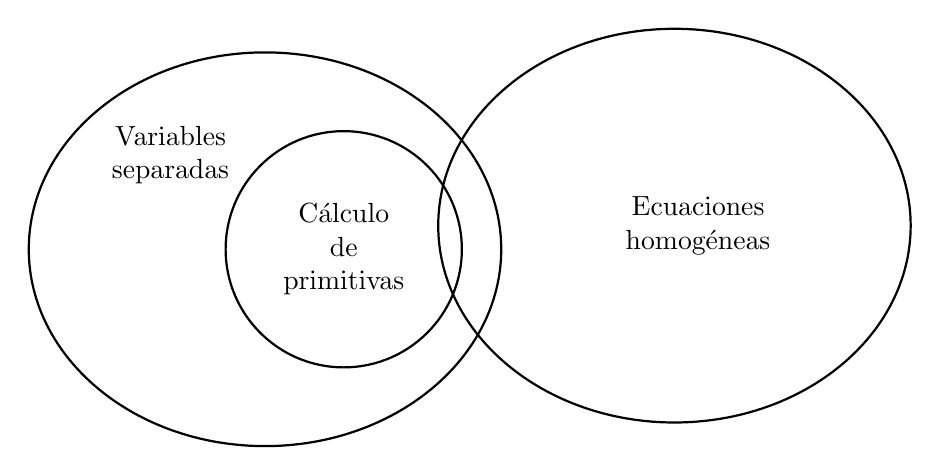
\begin{tikzpicture}
    % Conjunto B
    \draw[thick] (0,0) ellipse (3cm and 2.5cm);
    \node[align=center] at (-1.2,1.2) {Variables\\separadas}; % Salto de línea

    % Conjunto A (dentro de B)
    \draw[thick] (1,0) circle (1.5cm);
    \node[align=center] at (1,0) {Cálculo\\de\\primitivas}; % Salto de línea

    % Conjunto C
    \draw[thick] (5.2,0.3) ellipse (3cm and 2.5cm);
    \node[align=center] at (5.5,0.3) {Ecuaciones\\homogéneas}; % Salto de línea
\end{tikzpicture}
\caption{Diagrama de los tipos de ecuaciones diferenciales.}
\label{diag:tipos_ed}
\end{figure}

\subsubsection{Resolución de ecuaciones homoǵeneas}
Hay un cambio de variable que nos permite llevar ecuaciones diferenciales homogénes a ecuaciones diferenciales de variables separadas, que ya sabemos resolver. Por comodidad, supondremos que\footnote{En caso contrario, es análogo.} el dominio elegido para la ecuación diferencial es $D_+$.\\

El cambio viene dado por la función
\begin{equation*}
    \varphi : \left\{\begin{array}{rl}
            s &= t \\
            y &= \dfrac{x}{t}
    \end{array}\right.
\end{equation*}
\begin{itemize}
    \item Podemos despejar de manera única las variables $t$ y $x$, luego es biyectiva, con inversa:
\begin{equation*}
    \psi : \left\{\begin{array}{rl}
            t &= s \\
            x &= s y
    \end{array}\right.
\end{equation*}
    \item Las componentes $\varphi_1$ y $\varphi_2$ de $\varphi$ son polinomios, luego es de clase $C^1(D_+, \mathbb{R}^2)$.
    \item Y además, como las componentes $\psi_1$ y $\psi_2$ de $\psi$ también son polinomios, tenemos que $\psi$ es de clase $C^1(\varphi(D_+), \mathbb{R}^2)$.
\end{itemize}
Por tanto, hemos comprobado que $\varphi$ es un $C^1$-difeomorfismo, luego falta comprobar la condición de admisibilidad para comprobar que sea un cambio de variable admisible. Sin embargo, esta propiedad estará garantizada, ya que no hemos cambiado la variable $t$, por lo que:
\begin{equation*}
    \dfrac{\partial\varphi_1}{\partial t}(t,x) + \dfrac{\partial\varphi_1}{\partial x}(t,x) f(t,x) = 1 + 0 \neq 0 \qquad \forall (t,x)\in D_+
\end{equation*}

\noindent
Una vez comprobado que $\varphi$ es un cambio de variable admisible, vemos cuál será el nuevo dominio de la ecuación diferencial una vez hecho el cambio de variable:
\begin{equation*}
    \varphi(D_+) = \varphi\left(\left\{(t,x)\in \mathbb{R}^2 \mid t > 0, \dfrac{x}{t}\in J\right\}\right) = \left\{(s,y)\in \mathbb{R}^2 \mid s > 0, y\in J\right\} = \left]0, +\infty\right[ \times J
\end{equation*}
Por tanto, el sector angular $D_+$ que teníamos como dominio de la ecuación diferencial original, se aplica mediante $\varphi$ en una banda horizontal, tal y como vemos en la figura~\ref{fig:banda_horizontal}.

\begin{figure}[H]
\centering
\begin{tikzpicture}
    % Ejes coordenados
    \draw[-Stealth] (-0.5,0) -- (5,0) node[right] {$s$}; % Eje x
    \draw[-Stealth] (0,-0.5) -- (0,5) node[above] {$y$}; % Eje y

    % Recta y = \alpha
    \draw[thick] (-0.5,1) -- (5,1) node[right] {$y = \alpha$}; % Cambia 1 por el valor que desees para alpha

    % Recta y = \beta
    \draw[thick] (-0.5,3) -- (5,3) node[right] {$y = \beta$};  % Cambia 3 por el valor que desees para beta
    
    % Relleno de la banda entre y = \alpha y y = \beta
    \fill[blue!20, opacity=0.5] (0,1) rectangle (5,3);

\end{tikzpicture}
\caption{Banda horizontal, sin incluir la recta $s = 0$.}
\label{fig:banda_horizontal}
\end{figure}
Procederemos ahora a realizar el cambio de variable, para ver qué forma adopta la ecuación. Teníamos la ecuación
\begin{equation*}
    \dfrac{dx}{dt} = h\left(\dfrac{x}{t}\right)
\end{equation*}

a la que le aplicamos el cambio
\begin{equation*}
    \left\{\begin{array}{rl}
            s &= t \\
            y &= \dfrac{x}{t}
    \end{array}\right.
\end{equation*}

Pensando que $x$ está en función de $t$ y que $y$ está en función de $s$:
\begin{equation*}
    \dfrac{dy}{ds} = \dfrac{dy}{dt}\cancelto{1}{\dfrac{dt}{ds}} \AstIg \dfrac{t\cdot \dfrac{dx}{dt}-x}{t^2} = \dfrac{1}{t}\cdot \dfrac{dx}{dt} - \dfrac{1}{t}\cdot \dfrac{x}{t} = \dfrac{1}{t} \left(\dfrac{dx}{dt}-\dfrac{x}{t}\right)
\end{equation*}
Donde en $(\ast)$ hemos aplicado que $y = \frac{x}{t}$, junto con la regla de derivación de un cociente. Tenemos ya la ecuación diferencial, pero sigue estando en función de las variables $x$ y $t$. Falta aplicar que $y=\frac{x}{t}$ otra vez, que $s=t$ y que $x$ era solución de la ecuación diferencial, por lo que se verifica:
\begin{equation*}
    \dfrac{dx}{dt} = h\left(\dfrac{x}{t}\right)
\end{equation*}
Aplicando esto:
\begin{equation*}
    \dfrac{dy}{ds} = \dfrac{1}{t}\left(\dfrac{dx}{dt}-\dfrac{x}{t}\right) = \dfrac{1}{t}\left(h\left(\dfrac{x}{t}\right) - \dfrac{x}{t}\right) = \dfrac{1}{s}(h(y)-y)
\end{equation*}
Que es una ecuación de variables separadas, para las funciones\footnote{El dominio de la primera es $\mathbb{R}^+$ porque es el mismo dominio en el que se mueve $t$ y el de la segunda es el dominio en el que se mueve $\frac{x}{t}$.} $p:\mathbb{R}^+\rightarrow\mathbb{R}$ y $q:J\rightarrow\mathbb{R}$ dadas por:
\begin{gather*}
    p(s) = \dfrac{1}{s} \\
    q(y) = h(y) -y
\end{gather*}
Luego acabamos de ver que toda ecuación homogénea puede llevarse a una ecuación de variables separadas.\\

Recordamos que en variables separadas podíamos encontrarnos dos tipos de soluciones, constantes y no constantes. Observemos que cuando $q(b)=h(b)-b=0$ para cierto $b$, encontramos soluciones constantes de la ecuación diferencial de variables separadas, que serán las funciones:
\begin{equation*}
    z(s) = b \qquad \forall s\in \mathbb{R}^+
\end{equation*}
Que al deshacer el cambio de variable, nos darán una semirrecta en el dominio original:
\begin{equation*}
    x(t) = b\cdot t \qquad \forall t\in \mathbb{R}^+
\end{equation*}~\\
Resumiendo, dada una ecuación diferencial en un dominio $D_+$ por:
\begin{equation*}
    x' = h\left(\dfrac{x}{t}\right)
\end{equation*}
para cierta $h:J\rightarrow\mathbb{R}$ continua, podemos aplicar el cambio de variable
\begin{equation*}
    \left\{\begin{array}{rl}
            s &= t \\
            y &= \dfrac{x}{t}
    \end{array}\right.
\end{equation*}
para llegar a la ecuación diferencial de variables separadas
\begin{equation*}
    y' = \dfrac{1}{s}(h(y)-y)
\end{equation*}
que ya sabemos resolver.

\begin{ejemplo}
    Dada la ecuación diferencial (en la que usamos la notación geométrica en lugar de la física):
    \begin{equation*}
        y' = \dfrac{y-x}{y+x}
    \end{equation*}
    Se pide hallar su dominio de definición, así como encontrar una solución de dicha ecuación, cogiendo como condición de dicha solución que ha de cumplir: 
    \begin{equation*}
        y(-1) = -1
    \end{equation*}
    Se trata de una ecuación diferencial homogénea, ya que se trata de un cociente de dos polinomios homogéneos de grado 1. Podemos comprobarlo dividiendo numerador y denominador entre $x$:
    \begin{equation*}
        y' = \dfrac{y-x}{y+x} = \dfrac{\dfrac{y-x}{x}}{\dfrac{y+x}{x}} = \dfrac{\dfrac{y}{x}-1}{\dfrac{y}{x}+1}
    \end{equation*}
    Por lo que la función $h$ a escoger sería:
    \begin{equation*}
        h(\xi) = \dfrac{\xi - 1}{\xi + 1}
    \end{equation*}
    Y debemos elegir bien el dominio de definición de dicha función. Podría ser o bien $J_- = \left]-\infty, -1\right[$ o bien $J_+ = \left]-1, +\infty\right[$.\\
    Como queremos que $y(-1) = -1$, buscamos tener $\dfrac{y}{x} = \dfrac{-1}{-1}=  1$, luego tomaremos $J = J_+$, ya que contiene el 1.\\

    Una vez conocido el dominio de $h$, podemos ya escoger el dominio de definición de la ecuación diferencial. Este será $D_+$ o $D_-$. Como ha de cumplir que $(-1,-1)\in D$ siendo $D$ el dominio de la ecuación diferencial, nos quedaremos con $D = D_-$, ya que es la opción que nos contiene las abscisas negativas. De esta forma:
    \begin{equation*}
        D = \left\{(x,y)\in \mathbb{R}^2 \mid x<0, \dfrac{y}{x}>-1\right\}
    \end{equation*}
    Gráficamente, el dominio de definición $D$ es el sector angular de la figura~\ref{graph:sector_angular_ejercicio}.

\begin{figure}[H]
\centering
\begin{tikzpicture}
    % Ejes coordenados
    \draw[-Stealth] (-5,0) -- (1,0) node[right] {$x$};
    \draw[-Stealth] (0,-2) -- (0,3) node[above] {$y$};

    % Recta y = -x
    \draw[thick, dashed] (-4,4) -- (0,0) node[above=30] {};

    \filldraw[red] (-1,-1) circle (2pt) node[below left] {(-1,-1)};

    % Región sombreada donde x < 0 y y > -x
    \fill[blue!20, opacity=0.5] (-4,4) -- (0,0) -- (-4,0) -- cycle;
    \fill[blue!20, opacity=0.5] (-4,0) rectangle (0,-2);
\end{tikzpicture}
\caption{El sector angular $D$.}
\label{graph:sector_angular_ejercicio}
\end{figure}
\noindent
    Ahora, haremos el cambio de variable, usando como nuevas variables $u$ y $v$:
    \begin{equation*}
        \varphi: \left\{\begin{array}{rl}
                u &= x \\
                v &= \dfrac{y}{x}
        \end{array}\right.
    \end{equation*}
    De esta forma, el conjunto $D$ pasa a:
    \begin{equation*}
        \varphi(D) = \{(u,v)\in \mathbb{R}^2 \mid u < 0, v > -1\} = \left]-\infty, 0\right[ \times \left]-1,+\infty\right[
    \end{equation*}
    Y el punto $(-1,-1)$ pasa a:
    \begin{equation*}
        \varphi(-1,-1) = \left(-1, \dfrac{-1}{-1}\right) = (-1, 1)
    \end{equation*}
    Gráficamente, vemos $\varphi(D)$ en la figura~\ref{graph:banda_horizontal_ejercicio}.

\begin{figure}%[H]
\centering
\begin{tikzpicture}
    % Ejes coordenados
    \draw[-Stealth] (-5,0) -- (1,0) node[right] {$u$};
    \draw[-Stealth] (0,-1) -- (0,3) node[above] {$v$};

    % Recta y = -1
    \draw[thick, dashed] (0,-1) -- (-5,-1) node[above=30] {};

    \filldraw[red] (-1,1) circle (2pt) node[below left] {(-1,1)};

    % Región sombreada donde x < 0 y y > -x
    \fill[blue!20, opacity=0.5] (0,-1) rectangle (-5,3);
\end{tikzpicture}
\caption{Dominio tras hacer el cambio de variable}
\label{graph:banda_horizontal_ejercicio}
\end{figure}

\noindent
Buscamos ahora la ecuación diferencial tras el cambio de variable, la cual resulta en:
\begin{align*}
    \dfrac{dv}{du} &= \dfrac{dv}{dx} \cancelto{1}{\dfrac{dx}{du}} = \dfrac{x\dfrac{dy}{dx}-y}{x^2} = \dfrac{1}{x} \left( \dfrac{dy}{dx} - \dfrac{y}{x} \right) = \dfrac{1}{u}(h(v)-v) = \dfrac{1}{u}\left(\dfrac{v-1}{v+1}-v\right) \\
                   &= \dfrac{1}{u}\left(\dfrac{v-1}{v+1}-\dfrac{v^2+v}{v+1}\right) = \dfrac{-1}{u}\cdot \dfrac{1+v^2}{1+v}
\end{align*}
Y tenemos nuestra ecuación de variables separadas, que pasamos a resolver. Lo primero a observar es que nos interesa la solución concreta $v$ tal que $v(-1)=1$.\\

 Observamos que la ecuación anterior no tienen soluciones constantes, por ser:
 \begin{equation*}
     \dfrac{1+v^2}{1+v} > 0
 \end{equation*}

 Luego resolvemos por variables separadas:
 \begin{gather*}
     \dfrac{dv}{du} = \dfrac{-1}{u}\cdot \dfrac{1+v^2}{1+v} \\
     \int \dfrac{1+v}{1+v^2}~dv = -\int \dfrac{du}{u}
 \end{gather*}
 Como estamos trabajando con $u<0$:
 \begin{equation*}
     -\int \dfrac{du}{u}= -\ln(-u) + k
 \end{equation*}
 Y la primera integral la partimos en dos para resolverla, llegando a que:
 \begin{equation*}
     \int \dfrac{1+v}{1+v^2}~dv = \int \dfrac{1}{1+v^2}~dv + \int \dfrac{v}{1+v^2}~dv   = \arctg v +\dfrac{1}{2}\ln(1+v^2)
 \end{equation*}
 Por tanto:
 \begin{equation*}
     \arctg v + \dfrac{1}{2}\ln(1+v^2) = -\ln(-u) + k
 \end{equation*}
 Y por el desarrollo teórico visto en la sección de ecuaciones de variables separables, sabemos que dicha expresión define de forma implícita una función $v$ en función de $u$, para cierto $k\in \mathbb{R}$.

 \noindent
 Ahora, volveremos al dominio original, deshaciendo el cambio de variable:
 \begin{equation*}
     \arctg\left(\dfrac{y}{x}\right) + \dfrac{1}{2}\ln\left(1+\dfrac{y^2}{x^2}\right) = -\ln(-x) + k
 \end{equation*}
 Que define $y$ como función de $x$ de forma implícita. Usando que ($x<0$):
 \begin{equation*}
     \ln(-x) = \dfrac{1}{2}\ln\left(x^2\right)
 \end{equation*}
 Podemos darle otra forma a la expresión, para verla de forma más clara:
 \begin{equation*}
     \arctg\left(\dfrac{y}{x}\right) + \ln\left(\sqrt{x^2+y^2}\right) = k
 \end{equation*}
Es la familia de soluciones que nos resuelven la ecuación diferencial. Buscamos $k$ para $y(-1)=-1$, sustituyendo $y$ y $x$ por $-1$:
\begin{equation*}
    k = \dfrac{\pi}{4} + \ln\left(\sqrt{2}\right)
\end{equation*}
Para ver que esto define una ecuación implícita, deberíamos aplicar el Teorema, pero gracias a la teoría que venimos desarrollando hasta ahora, lo tenemos visto.
Tenemos visto que dicha fórmula dos define una ecuación implícita en un entorno del punto $(-1,-1)$.\\

\noindent
Sin embargo, estamos ante un problema específico en el que podemos llegar a ver algo más.
Se trata de una curva que en cartesianas tiene una expresión compleja, pero en coordenadas polares puede intuirse la gráfica de la función de forma más fácil, por lo que cambiamos a coordenadas polares:
\begin{equation*}
    \left\{\begin{array}{rl}
            x &= r\cos \theta \\
            y &= r\sen \theta
    \end{array}\right.
\end{equation*}
Y como:
\begin{equation*}
    \dfrac{y}{x} = \dfrac{r\sen\theta}{r\cos\theta}=  \tan \theta
\end{equation*}
Buscamos $\theta$ de forma que $\tan\theta = \frac{y}{x}$. Como estamos trabajando con la solución que pasa por el $(-1,-1)$, estamos trabajando en el tercer cuadrante, por lo que tendremos $\theta \in \left]\frac{\pi}{2}, \frac{3\pi}{2}\right[$. Como la función $\arctan$ es la inversa de $\tan$ sólo en el intervalo $\left]\frac{-\pi}{2},\frac{\pi}{2}\right[$, desplazamos $\theta$, usando que la tangente es $\pi$-periódica:
\begin{gather*}
    \theta \in \left]\frac{\pi}{2}, \frac{3\pi}{2}\right[ \Longrightarrow \theta -\pi \in \left]\frac{-\pi}{2},\frac{\pi}{2}\right[ \\
    \arctan(\tan \theta) = \arctan(\tan(\theta - \pi)) = \theta - \pi
\end{gather*}

Luego:
\begin{gather*}
    \arctan(\tan \theta) = \arctan\left(\dfrac{y}{x}\right) = \theta - \pi \\
    \theta = \arctan\left(\dfrac{y}{x}\right) + \pi
\end{gather*}

Y también:
\begin{equation*}
    r = \sqrt{x^2 + y ^2}
\end{equation*}
Finalmente, llegamos a que la expresión en polares es:
\begin{equation*}
    \theta + \ln r = k + \pi
\end{equation*}
Se trata de la espiral logarítmica o de Arquímedes, que se entiende mejor tomando exponenciales:
\begin{equation*}
    r = e^{k-\theta+\pi}
\end{equation*}
Fijado un $r$, conforme movemos $\theta$, se va formando una especie de circunferencia pero con $r$ disminuyendo, luego se forma una espiral.
\begin{figure}[H]
\centering
\begin{tikzpicture}
    \begin{polaraxis}[
        domain=0:720,  % Ángulo en grados
        samples=500,   % Número de muestras (mejora la resolución)
        axis lines=none, % Ocultar los ejes
        ticks=none,    % Ocultar las marcas de los ejes
    ]
    % Graficar la espiral: r = a * exp(b * theta)
    \addplot[blue, thick] {0.5*exp(0.02*x)}; % a = 0.5, b = 0.02
    \end{polaraxis}
\end{tikzpicture}
\caption{Espiral logarítmica.}
\end{figure}
\end{ejemplo}

\begin{observacion}
Notemos que las espirales son curvas de la forma
\begin{equation*}
    r = f(\theta)
\end{equation*}
con $f$ creciente o decreciente, escritas en coordenadas polares.
\end{observacion}

\section{Ecuaciones reducibles a homogéneas}
A continuación, estudiaremos otro tipo de ecuaciones diferenciales, las reducibles a homogéneas. Estas son similares a las homogéneas, pero en vez de ser una función en función de $\frac{x}{t}$, es una función en función de un cociente de polinomios en dos variables, ambos de grado 1, luego son de la forma:
\begin{equation*}
    x' = h\left(\dfrac{at + bx + c}{At + Bx + C}\right) \qquad a,b,c,A,B,C \in \mathbb{R}
\end{equation*}

con $h:I\rightarrow\mathbb{R}$ una función continua con $I$ un intervalo abierto.

\begin{ejercicio*}
    Dar un dominio de definición para una ecuación reducible a homogénea.

Estaremos trabajando por tanto con una ecuación diferencial de la forma
\begin{equation*}
    x' = f(t,x)
\end{equation*}

con
\begin{equation*}
    f(t,x) = h\left(\dfrac{at + bx + c}{At + Bx + C}\right) \qquad a,b,c,A,B,C \in \mathbb{R}, \quad \forall (t,x)\in D
\end{equation*}
Y buscamos el dominio $D$ en el que la función $f$ está definida. Este tiene que ser un conjunto abierto y conexo de $\mathbb{R}^2$.\\

Dado $(t,x)\in \mathbb{R}^2$, nos interesa:
\begin{itemize}
    \item Primero, que el cociente anterior tenga sentido, es decir, que $At + Bx + C \neq 0$. Por tanto, esta recta estará excluida de $D$.
    \item Que podamos aplicar $h$ al cociente anterior, es decir, que
        \begin{equation*}
            \dfrac{at + bx + c }{At + Bx + C} \in I
        \end{equation*}
\end{itemize}
El conjunto más grande en el que podemos definir $f$ será un conjunto de la forma:
\begin{equation*}
    D = \left\{(t,x)\in \mathbb{R}^2 \mid At + Bx + C \neq 0, \dfrac{at + bx + c }{At + Bx + C} \in I \right\}
\end{equation*}
Finalmente, falta comprobar que el conjunto sea abierto y conexo. Como el conjunto excluye a una recta del plano, sabemos por tanto que este contendrá como mínimo dos componentes conexas\footnote{Si algún lector termina el ejercicio, solicitamos que se nos envíe para completar los aputnes.}.
\end{ejercicio*}

\subsubsection{Resolución de ecuaciones reducibles a homogéneas}
\noindent
El truco que funciona casi siempre es realizar una traslación. Fijado $(t_*, x_*)\in \mathbb{R}^2$, defino
\begin{equation*}
    \varphi: \left\{\begin{array}{rl}
            s &= t - t_* \\
            y &= x - x_*
    \end{array}\right. \qquad (t_*, x_*)\in \mathbb{R}^2
\end{equation*}

que es fácil ver que es un cambio de variable admisible.

El cambio de variable es:
\begin{equation*}
    \dfrac{dy}{ds} = \dfrac{dx}{dt} = f(t,x)
\end{equation*}

Y hay que quitar las variables $t$ y $x$:
\begin{equation*}
    \dfrac{dy}{ds} = h\left(\dfrac{a(s+t_*)+b(y+x_*)+c}{A(s+t_*)+B(y+x_*)+C}\right)
\end{equation*}

Si conseguimos hacer:
\begin{gather*}
    \left\{\begin{array}{ll}
            at_* + bx_* + c &= 0 \\
        At_* + Bx_* + C &= 0
    \end{array}\right.
\end{gather*}
Nos quedaría que:
\begin{equation*}
    \dfrac{dy}{ds} = h\left(\dfrac{a(s+t_*)+b(y+x_*)+c}{A(s+t_*)+B(y+x_*)+C}\right) = h\left(\dfrac{as + by}{As+By}\right)
\end{equation*}
Que se trata de una ecuación homogénea, por ser un cociente de polinomios homogéneos de grado 1.\\

\begin{itemize}
    \item En el caso de que
        \begin{equation*}
            \left|\begin{array}{cc}
                a & b \\
                A & B
            \end{array}\right| \neq 0
        \end{equation*}
        Entonces, el sistema anterior es compatible determinado, por lo que existe una solución del sistema. Para realizar el cambio de variable, tomamos $(t_*,x_*)$ de forma que sea solución del sistema, y al realizar el cambio de variable, podremos seguir el razonamiento superior, llegando a una ecuación homogénea.
    \item En el caso de que
        \begin{equation*}
            \left|\begin{array}{cc}
                a & b \\
                A & B
            \end{array}\right| = 0
        \end{equation*}
        Entonces, se trata de un sistema incompatibles, por lo que no podremos realizar el razonamiento anterior.

        Sin embargo, lo que sucederá en dicho caso es que los vectores $(a,b)$ y $(A,B)$ serán linealmente dependientes en $\mathbb{R}^2$, luego podemos hacer:
        \begin{equation*}
            (A,B) = \lm(a,b) \qquad \lm \in \mathbb{R}
        \end{equation*}
        De esta forma, podemos escribir:
        \begin{equation*}
            x' = h\left(\dfrac{at + bx + c}{At + Bx + C}\right) =  h\left(\dfrac{at + bx + c}{\lm(at+bx)+c}\right) 
        \end{equation*}
        Que no es una ecuación homogénea, pero nos permite hacer el cambio de variable (suponiendo que $b\neq 0$):
    \begin{equation*}
        y = at + bx 
    \end{equation*}
\end{itemize}

%\begin{ejemplo}
%    Un problema que podemos encontrarnos es:
%    \begin{equation*}
%        x' = \dfrac{x+t+1}{x-t+3}\qquad x(0)=0
%    \end{equation*}
%    Encuentre la solución a este problema y diga en qué intervalo está definido.\\
%
%    Primero, comenzaremos viendo en qué dominio está definida la ecuación diferencial. Para ello, buscamos un conjunto $D\subseteq \mathbb{R}^2$ abierto y conexo en el que $f$ (función que nos da la forma normal) sea una función continua.\\
%
%    Para que $f$ sea continua, basta con que esté definida en un conjunto que no contenga ningún punto de la recta $x-t+3 = 0$. Esta nos divide el plano en dos componentes conexas, por lo que los dominios que podemos tomar para definir la función $f$ de forma que estos sean conexos y abiertos son:
%    \begin{gather*}
%        D_+ = \{(t,x)\in \mathbb{R}^2 \mid x-t+3 < 0\} \\
%        D_- = \{(t,x)\in \mathbb{R}^2 \mid x-t+3 > 0\} 
%    \end{gather*}
%    Hemos de quedarnos con uno de ellos. Como nos interesa buscar la solución $x=x(t)$ que cumpla $x(0)=0$, nos intersa que en nuestro dominio de definición de $f$ se encuentre el punto $(0,0)$. Nos quedamos por tanto con el dominio $D = D_-$ (ya que $0-0+3>0$).
%
%\begin{figure}[H]
%\centering    
%\begin{tikzpicture}
%    % Dibujar los ejes
%    \draw[-Stealth] (5,0) -- (-1,0) node[left] {$t$};
%    \draw[-Stealth] (0,-4) -- (0,1) node[above] {$x$};
%    
%    % Dibujar la recta y = x - 3
%    \draw[domain=-1:4, thick, grey] plot (\x, {(\x - 3)}) node[right] {$x-t+3=0$};
%    \filldraw[red] (0,0) circle (2pt) node[below left] {(0,0)};
%\end{tikzpicture}
%\caption{Regiones del plano divididas por la recta $x-t+3=0$.}
%\label{fig:sector_angular}
%\end{figure}
%Por tanto, nos interesa resolver la ecuación diferencial
%\begin{equation*}
%    x' = f(t,x)
%\end{equation*}
%
%con $f:D_-\rightarrow\mathbb{R}$ una función continua con
%\begin{equation*}
%    f(t,x) = \dfrac{x+t+1}{x-t+3} \qquad  (t,x)\in D_-
%\end{equation*}
%Observemos que se trata de una ecuación reducible a homogénea, y como:
%\begin{equation*}
%    \left|\begin{array}{cr}
%            1 & 1 \\
%            1 & -1
%    \end{array}\right| = -2 \neq 0
%\end{equation*}
%Entonces, el sistema
%\begin{equation*}
%    \left\{\begin{array}{rl}
%            x + t + 1 &= 0 \\
%            x - t + 3 &= 0
%    \end{array}\right.
%\end{equation*}
%es compatible determinado. Lo resolvemos con vistas a aplicar el cambio de variable que hemos visto que funciona:
%\begin{gather*}
%    \left\{\begin{array}{rlcl}
%            x + t + 1 &= 0 & \Longrightarrow & t = -x - 1 \\
%            x - t + 3 &= 0 & \Longrightarrow & 2x+4=0 \Longrightarrow x=-2
%    \end{array}\right.\\
%    t= -x-1 \Longrightarrow t = 2-1 = 1
%\end{gather*}
%Obtenemos el punto $(t_*, x_*) = (1, -2)$. Realizamos el cambio de variable:
%\begin{equation*}
%    \varphi: \left\{\begin{array}{rl}
%            s &= t - 1 \\
%            y &= x + 2
%    \end{array}\right.
%\end{equation*}
%Obteniendo la ecuación diferencial:
%\begin{equation*}
%    \dfrac{dy}{ds} = \dfrac{dx}{dt} = \dfrac{x+t+1}{x-t+3}
%\end{equation*}
%Despejando $x$ y $t$ del cambio:
%\begin{equation*}
%    \left\{\begin{array}{rl}
%            t &= s+1 \\
%            x &= y-2
%    \end{array}\right.
%\end{equation*}
%\begin{equation*}
%    \dfrac{dy}{ds} = \dfrac{x+t+1}{x-t+3} = \dfrac{y-2+s+1+1}{y-2-s-1+3} = \dfrac{y+s}{y-s}
%\end{equation*}
%Que ahora estará definida en:
%\begin{equation*}
%    D_-^* = \varphi(D_-) = \{(s,y)\in \mathbb{R}^2 \mid y-2-s-1+3 > 0 \} =  \{(s,y)\in \mathbb{R}^2 \mid y-s > 0 \} 
%\end{equation*}
%Y nos interesará el punto $\varphi(0,0) = (-1,2)$.
%
%\begin{figure}[H]
%\centering    
%\begin{tikzpicture}
%    % Dibujar los ejes
%    \draw[-Stealth] (3,0) -- (-3,0) node[left] {$s$};
%    \draw[-Stealth] (0,-3) -- (0,3) node[above] {$y$};
%    
%    % Dibujar la recta y = x - 3
%    \draw[domain=-3:3, thick, grey] plot (\x, {\x}) node[right] {$y-s=0$};
%    \filldraw[red] (-1,2) circle (2pt) node[below left] {(-1,2)};
%\end{tikzpicture}
%\caption{Regiones del plano divididas por la recta $y-s=0$.}
%\end{figure}
%
%Tenemos la ecuación
%\begin{equation*}
%    \dfrac{dy}{ds} = \dfrac{y+s}{y-s}
%\end{equation*}
%Que es una ecuación homogénea, por ser cociente de polinomios homogéneos de grado 1. Obtenemos la función $h$, dividiendo entre $s$:
%\begin{equation*}
%    \dfrac{y+s}{y-s} = \dfrac{\dfrac{y+s}{s}}{\dfrac{y-s}{s}} = \dfrac{\dfrac{y}{s}+1}{\dfrac{y}{s}-1}
%\end{equation*}
%Luego tenemos la ecuación homogénea
%\begin{equation*}
%    \dfrac{dy}{ds} = h\left(\dfrac{y}{s}\right)
%\end{equation*}
%
%con $h:I=\left]-\infty,1\right[\rightarrow\mathbb{R}$ dada por
%\begin{equation*}
%    h(\xi) = \dfrac{\xi+1}{\xi -1}
%\end{equation*}
%donde hemos cogido el dominio $\left]-\infty, 1\right[$ en vez de $\left]1,+\infty\right[$ ya que nos interesa tener al punto $(-1,2)$, el cual cumple que:
%\begin{equation*}
%    \dfrac{y}{s} = \dfrac{2}{-1} = -2 < 1
%\end{equation*}
%En definitiva, estamos trabajando ahora con la ecuación diferencial
%\begin{equation*}
%    \dfrac{dy}{ds} = \dfrac{y+s}{y-s}
%\end{equation*}
%definida en $D_-^*$, pero para resolverla hemos de considerar que $s\neq 0$, para poder dividir, por lo que hemos de excluir del dominio la recta $s=0$. Esta nos divide el semiplano en dos componentes conexas, como observamos en la figura~\ref{graph:ejm_reducibles}.
%\begin{figure}[H]
%\centering    
%\begin{tikzpicture}
%    % Dibujar los ejes
%    \draw[-Stealth] (3,0) -- (-3,0) node[left] {$s$};
%    \draw[-Stealth] (0,-3) -- (0,3) node[above] {$y$};
%    
%    % Dibujar la recta y = x - 3
%    \draw[domain=-3:3, thick, grey] plot (\x, {\x}) node[right] {$y-s=0$};
%    \draw[thick, blue] (0,-3) -- (0,3) node[below right] {$s=0$};
%    \filldraw[red] (-1,2) circle (2pt) node[below left] {(-1,2)};
%\end{tikzpicture}
%\caption{Regiones del semiplano divididas por la recta $s=0$.}
%\label{graph:ejm_reducibles}
%\end{figure}
%Estas compoentes son:
%\begin{gather*}
%    A_1 = \{(s,y) \in \mathbb{R}^2 \mid y-s > 0, s < 0\} \\
%    A_2 = \{(s,y) \in \mathbb{R}^2 \mid y-s > 0, s > 0\} \\
%\end{gather*}
%Nos quedamos con $A_1$, ya que nos interesa que la solución contenga al punto $(-1,2)$, que se encuentra en $A_1$. Notemos que este es uno de los sectores angulares que obtenemos como resultado de escoger el dominio anterior para la función $h$.
%
%Ahora, estamos listos para aplicar el cambio de variable que nos lleva esta ecuación homogénea en una de variable separadas. Realizaremos el cambio:
%\begin{equation*}
%    \alpha: \left\{\begin{array}{rl}
%            u &= s \\
%            v &= \dfrac{y}{s}
%    \end{array}\right.
%\end{equation*}
%
%llegando a la ecuación:
%\begin{align*}
%    \dfrac{dv}{du} &= \dfrac{dv}{ds} = \dfrac{s\cdot  \dfrac{dy}{ds}-y}{s^2} = \dfrac{1}{s}\cdot \dfrac{dy}{ds} - \dfrac{1}{s}\cdot \dfrac{y}{s}= \dfrac{1}{s} \left(\dfrac{dy}{ds} - \dfrac{y}{s}\right) = \dfrac{1}{s} \left(\dfrac{y+s}{y-s}-\dfrac{y}{s}\right)\\
%                   &= \dfrac{1}{s}\left(\dfrac{\dfrac{y}{s}+1}{\dfrac{y}{s}-1}-\dfrac{y}{s}\right) = \dfrac{1}{u}\left(\dfrac{v+1}{v-1}-v\right) = \dfrac{1}{u}\left(\dfrac{-v^2 + 2v +1 }{v-1}\right)
%\end{align*}
%Que es de variables separadas. Buscamos ahora su dominio. Como:
%\begin{equation*}
%    A_1 = \{(s,y) \in \mathbb{R}^2 \mid y-s > 0, s < 0\} = \left\{(s,y)\in \mathbb{R}^2 \mid \dfrac{y}{s}<1, s<0\right\}
%\end{equation*}
%
%Entonces:
%\begin{equation*}
%    \alpha(A_1) = \{(u,v)\in \mathbb{R}^2 \mid v < 1, u < 0\} = \mathbb{R}^- \times I
%\end{equation*}
%Pasamos a resolver la ecuación de variables separadas:
%
%\begin{itemize}
%    \item Soluciones constantes:
%        \begin{equation*}
%            \dfrac{-v^2 +2v+1}{v-1} = 0 \Longleftrightarrow v = 1\pm \sqrt{2}
%        \end{equation*}
%    \item Para aquellos puntos en los que no se anule:
%        \begin{gather*}
%            \dfrac{dv}{du} =  \dfrac{1}{u}\left(\dfrac{-v^2 + 2v +1 }{v-1}\right) \\
%            \dfrac{dv}{\dfrac{-v^2 +2v+1}{v-1}} = \dfrac{v-1}{-v^2 +2v+1}~dv =\dfrac{du}{u} \\
%            \int \dfrac{v-1}{-v^2 +2v+1}~dv = \int \dfrac{du}{u} \\
%            c+\dfrac{-1}{2} \ln(|-v^2 +2v+1|) = \ln (-u) \\
%            c = \ln\left(-u \sqrt{|-v^2 +2v+1|}\right) \\
%            e^c = -u \sqrt{|-v^2 + 2v+1|}
%        \end{gather*}
%\end{itemize}
%
%\end{ejemplo}

\section{Ecuaciones lineales}
Las ecuaciones diferenciales lineales son de la forma
\begin{equation*}
    x' = a(t)x + b(t)
\end{equation*}

para ciertas funciones $a,b:J\rightarrow\mathbb{R}$ continuas definidas en un intervalo abierto $J$.\\

\noindent
Por tanto, la ecuación diferencial vendrá dada por una función $f:J\times \mathbb{R}\rightarrow\mathbb{R}$ de forma que
\begin{equation*}
    x' = f(t,x) = a(t)x + b(t) \qquad (t,x)\in J\times \mathbb{R}
\end{equation*}
Observemos que el dominio de $f$ se trata de una banda vertical.\\

Las ecuaciones lineales pueden clasificarse en dos tipos:
\begin{itemize}
    \item Si $b(t)=0$ $\forall t\in J$, entonces estamos ante una ecuación lineal homogénea\footnote{no tiene nada que ver con las ecuaciones homogéneas}.
    \item Si $b$ no es la función constantemente igual a cero, decimos que es una ecuación lineal completa.
\end{itemize}

\begin{observacion}
Observemos que $x' = \frac{x}{t}$ es de variables separadas, homogénea, reducible a homogenea y lineal homogénea.
\end{observacion}

\subsection{Ecuaciones lineales homogeneas}
Como hemos comentado antes, se tratan de ecuaciones de la forma
\begin{equation*}
    x' = a(t) x
\end{equation*}
para $a:J\rightarrow\mathbb{R}$ una función continua definida en un intervalo abierto $J$. Este tipo de ecuaciones sabemos ya resolverlas, pues son ecuaciones de variables separadas:
\begin{equation*}
    x' = p(t)q(x)
\end{equation*}
Para las funciones $p:J\rightarrow\mathbb{R}$, $q:\mathbb{R}\rightarrow\mathbb{R}$ dadas por:
\begin{gather*}
    p(t) = a(t) \qquad t\in J \\
    q(x) = x \qquad x\in \mathbb{R}
\end{gather*}
Como $q(x) = 0\Longleftrightarrow x=0$, tenemos que sólo hay una solución constante:
\begin{equation*}
    x(t) = 0 \qquad t \in J
\end{equation*}
Para sacar el resto, hacemos separación de variables:
\begin{gather*}
    \dfrac{dx}{dt} = a(t) x \\
    \int \dfrac{dx}{x}~dx  = \int a(t)~dt
\end{gather*}
Y dependerá de que $x$ sea positivo o negativo para calcular la primera integral:
\begin{equation*}
    \int \dfrac{dx}{x}~dx  = \left\{\begin{array}{cl}
            \ln x & \text{si\ } x > 0 \\
            \ln (-x) & \text{si\ } x < 0 \\
    \end{array}\right.
\end{equation*}
Y notando por:
\begin{equation*}
    A(t) = \int_{t_0}^{t} a(s)~ds 
\end{equation*}

para cierto $t_0 \in I$, tenemos que:
\begin{itemize}
    \item Suponiendo que $x>0$:
        \begin{gather*}
            \ln x = A(t) + c \\
            x(t) = e^c e^{A(t)} \qquad t\in J
        \end{gather*}
        Luego las soluciones son de la forma:
        \begin{equation*}
            x(t) = k\cdot e^{A(t)} \qquad k\in \mathbb{R}^+, \quad t\in J
        \end{equation*}
    \item Suponiendo que $x<0$:
        \begin{gather*}
            \ln (-x) = A(t) + c \\
            x(t) = -e^c e^{A(t)} \qquad t\in J
        \end{gather*}
        Luego las soluciones son de la forma:
        \begin{equation*}
            x(t) = k\cdot e^{A(t)} \qquad k\in \mathbb{R}^-, \quad t\in J
        \end{equation*}
\end{itemize}
En definitiva, dada una ecuacion de la forma
\begin{equation*}
    x' = a(t)x\qquad t\in J
\end{equation*}
Entonces, sus soluciones son de la forma:
\begin{equation*}
    x(t) = k\cdot e^{A(t)} \qquad k\in \mathbb{R}, \quad t\in J
\end{equation*}

con
\begin{equation*}
    A(t) = \int_{t_0}^{t} a(s)~ds \qquad t\in J
\end{equation*}

para cierto $t_0\in J$.

\begin{ejemplo}
    Resolvamos
    \begin{equation*}
        x' = \dfrac{x}{t} \qquad t\in \mathbb{R}^-
    \end{equation*}
    Trabajaremos por tanto en el semiplano en el que $t<0$.\\

    En este caso, tenemos $a(t) = \frac{1}{t}$, por lo que:
    \begin{equation*}
        A(t) = \int_{t_0}^{t} \dfrac{1}{s}~ds  = \ln(-t)
    \end{equation*}

    para cierto $t_0\in \mathbb{R}^-$. Las soluciones de dicha ecuación serán:
    \begin{equation*}
        x(t) = k\cdot e^{\ln(-t)} = -k\cdot t \qquad k\in \mathbb{R}, \quad t\in \mathbb{R}^-
    \end{equation*}
\end{ejemplo}

\subsection{Ecuaciones lineales completas}
Son de la forma
\begin{equation}\label{eq:lineal_completa}
    x' = a(t)x + b(t)
\end{equation}
para ciertas funciones $a,b:J\rightarrow\mathbb{R}$ con $J$ un intervalo abierto de forma que la función $b$ no es constantemente igual a 0. Notaremos a su dominio $D = J\times \mathbb{R}$.\\

Resolveremos este tipo de ecuaciones mediante un cambio de variable, el cual pasamos a buscar. Dada una función $l:J\rightarrow\mathbb{R}$ con $l(t)\neq 0$ $\forall t\in J$ y $l \in C^1(J)$, definimos el cambio de variable:
\begin{equation*}
    \varphi: \left\{\begin{array}{rl}
            s &= t \\
            y &= l(t) x
    \end{array}\right.
\end{equation*}
Que tenemos que ver que es admisible:
\begin{itemize}
    \item $\varphi$ es de clase $C^1(D)$, ya que sus componentes $\varphi_1$ y $\varphi_2$ son de clase $C^1(D)$ ($\varphi_2$ es productor de funciones de clase $C^1(D)$).
    \item Despejando las variables $t$ y $x$ (gracias a que $l(t)\neq 0$ $\forall t\in J$), podemos dar una inversa $\psi$ de $\varphi$, por lo que es biyectiva:
        \begin{equation*}
            \psi: \left\{\begin{array}{rl}
                    t &= s \\
                    x &= \dfrac{y}{l(s)}
            \end{array}\right.
        \end{equation*}
        Es fácil ver que $\psi$ es inversa de $\varphi$.
    \item Observando las componentes $\psi_1$ y $\psi_2$, vemos que estas son de clase $C^1$, luego $\psi$ es de clase $C^1$. Tenemos ya probado que $\varphi$ es un difeomorfismo.
    \item Por ser $s = t$, tenemos garantizada la condición de admisibilidad, ya que:
        \begin{equation*}
            \dfrac{\partial\varphi_1}{\partial t}(t,x(t)) + \dfrac{\partial\varphi_1}{\partial x}(t,x(t)) f(t,x(t)) = 1 + 0 \neq 0 \qquad \forall t\in J
        \end{equation*}

    \item Finalmente, observemos que si $(t,x)\in D$, entonces $\varphi(t,x)\in D$, por lo que $\varphi(D) = D$:
        \begin{equation*}
            \varphi(t,x) = (t, l(t) x) \in J\times \mathbb{R} = D
        \end{equation*}
\end{itemize}
A continuación, aplicaremos dicha familia de cambios de variable (ya que por cada función $l$ tenemos un cambio de variable distinto) a la ecuación~\ref{eq:lineal_completa}:
\begin{equation*}
    \left\{\begin{array}{rl}
            s &= t \\
            y &= lx
    \end{array}\right.
\end{equation*}
entendiendo que todo son funciones dependientes de $t$:
\begin{equation*}
    y' = l' x + lx' = l'x + l(ax+b)
\end{equation*}

sustituimos $x$ por $\frac{y}{l}$:
\begin{equation*}
    y' = \dfrac{l'}{l}y + l\left(a\dfrac{y}{l}+b\right)
\end{equation*}
Y obtenemos otra ecuación diferencial lineal:
\begin{equation*}
    y' = \left(\dfrac{l'}{l} + a\right) y + bl
\end{equation*}
Sin embargo, podemos convertirlo en un cálculo de primitivas, buscando que:
\begin{equation*}
    \dfrac{l'}{l}+a = 0
\end{equation*}
Que podemos pensarlo como una ecuación diferencial para $l$:
\begin{equation*}
    l' = -a(t) l
\end{equation*}
Que es una ecuación lineal homogénea, cuyas soluciones sabemos ya que son de la forma: 
\begin{equation*}
    l(t) = k\cdot e^{-A(t)} \qquad k\in \mathbb{R},\quad t\in J
\end{equation*}
Escogemos la solución $l(t) = e^{-A(t)}$.\\

Por tanto, el resultado tras aplicar el cambio de variable con la función $l$ ahora conocida resulta en la ecuación diferencial
\begin{equation*}
    y' = b(t)l(t)
\end{equation*}
que la resolvemos mediante cálculo de primitivas:
\begin{equation*}
    y(t) = \int_{t_0}^{t} b(s)l(s)~ds + k
\end{equation*}

con nuestra función $l$:
\begin{equation*}
    y(t) = \int_{t_0}^{t} b(s)e^{-A(s)}~ds + k
\end{equation*}
Una vez obtenida $y$, sacamos las soluciones de las ecuaciones lineales completas, deshaciendo el cambio de variable $x=\frac{y}{l}$:
\begin{equation*}
    x(t) = ke^{A(t)} + e^{A(t)} \int_{t_0}^{t} e^{-A(s)}b(s)~ds 
\end{equation*}

\begin{ejemplo}
    Resolver la ecuación
    \begin{equation*}
        x' = \dfrac{x}{t} + 1
    \end{equation*}
    con $t<0$.\\

    Hacemos el cambio $y=l(t)x$, luego:
    \begin{equation*}
        y' = l'x + lx' = l' x + l\left(\dfrac{x}{t}+1\right) = \dfrac{l'}{l}y + l\left(\dfrac{\nicefrac{y}{l}}{t}+1\right)
    \end{equation*}
    \begin{equation*}
        y' = \left(\dfrac{l'}{l}+\dfrac{1}{t}\right) y + l
    \end{equation*}
    Buscamos una solución que cumpla:
    \begin{equation*}
        \dfrac{l'}{l}+\dfrac{1}{t} = 0
    \end{equation*}
    Es decir:
    \begin{equation*}
        l' = -\dfrac{l}{t}
    \end{equation*}
    No nos hacen falta todas las soluciones, simplemente una. Cogemos:
    \begin{equation*}
        l(t) = e^{-\ln(-t)} = \dfrac{-1}{t} \qquad t\in \mathbb{R}^-
    \end{equation*}

    tenemos que $l(t)\neq 0$ $\forall t\in \mathbb{R}^-$.\\

    Por tanto, tenemos:
    \begin{equation*}
        y' = l(t) = -\dfrac{1}{t}
    \end{equation*}
    \begin{equation*}
        y(t) = k - \ln(-t) \qquad k\in \mathbb{R}, \quad t\in \mathbb{R}^-
    \end{equation*}
    Luego:
    \begin{equation*}
        x(t) = -t\cdot (k-\ln(-t)) \qquad \forall k\in \mathbb{R}, \quad t\in \mathbb{R}^-
    \end{equation*}
\end{ejemplo}

\subsection{Ecuación de Riccati}
Podemos entender la ecuación lineal como una ecuación diferencial que simula ser un polinomio de primer grado. Riccati intentó solucionar aquella ecuación diferenial que simula ser un polinomio de segundo grado:
\begin{equation*}
    x' = a(t) x^2+b(t)x+c(t)
\end{equation*}
para ciertas $a,b,c:J\rightarrow\mathbb{R}$ funciones continuas definidas en un intervalo abierto $J$.
